% Aneva est une grosse cruchasse =D

\documentclass[a4paper]{article}

\usepackage[utf8]{inputenc} 
\usepackage[francais]{babel}  
\usepackage[T1]{fontenc}

\usepackage{graphicx}

\usepackage[top=2cm, bottom=2cm, left=2cm, right=2cm]{geometry}

\usepackage{hyperref}

% Headers and footers:
\usepackage{fancyhdr}
\pagestyle{fancy}
          \fancyhf{}
          \fancyfoot[LE,RO]{\thepage}
          % Rulers width
          \renewcommand{\footrulewidth}{.3pt}
          \renewcommand{\headrulewidth}{.3pt}
\fancyhead[RO,RE]{Johann Chazelle, Elisa Abidh, Sandra Mondain}
\fancyfoot[LO,RE]{Compte-rendu du TP Sherlock}

% Vars & functs
\newcommand\PIXPATH{../ressources}

\title{\vfill \textbf{Compte-rendu du TP Sherlock}}
\author{Johann \bsc{Chazelle}, Elisa \bsc{Abidh}, Sandra \bsc{Mondain}}
\date{16 décembre 2010\vfill}

\begin{document}

\maketitle

\newpage

\section{Modèle de maintenance}
Ici, acheter du terrain sur le TP et sur notre modèle de maintenance tout ça tout ça. 
\begin{figure}[!h]
\begin{center}
        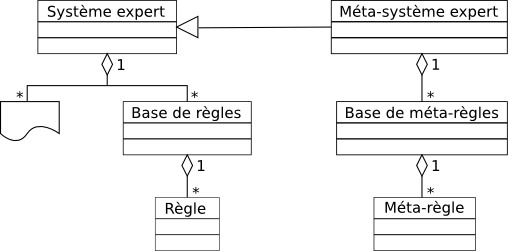
\includegraphics{\PIXPATH/Modele-Maintenance.png}
        \caption{Modèle de maintenance automatique de l'application Constat}
\end{center}
\end{figure}

\section{Réflexion sur la maintenance corrective et évolutive}
Terrain. 

\end{document}